\documentclass[11pt,a4paper,twoside]{report}\usepackage[]{graphicx}\usepackage[]{color}
% maxwidth is the original width if it is less than linewidth
% otherwise use linewidth (to make sure the graphics do not exceed the margin)
\makeatletter
\def\maxwidth{ %
  \ifdim\Gin@nat@width>\linewidth
    \linewidth
  \else
    \Gin@nat@width
  \fi
}
\makeatother

\definecolor{fgcolor}{rgb}{0.345, 0.345, 0.345}
\newcommand{\hlnum}[1]{\textcolor[rgb]{0.686,0.059,0.569}{#1}}%
\newcommand{\hlstr}[1]{\textcolor[rgb]{0.192,0.494,0.8}{#1}}%
\newcommand{\hlcom}[1]{\textcolor[rgb]{0.678,0.584,0.686}{\textit{#1}}}%
\newcommand{\hlopt}[1]{\textcolor[rgb]{0,0,0}{#1}}%
\newcommand{\hlstd}[1]{\textcolor[rgb]{0.345,0.345,0.345}{#1}}%
\newcommand{\hlkwa}[1]{\textcolor[rgb]{0.161,0.373,0.58}{\textbf{#1}}}%
\newcommand{\hlkwb}[1]{\textcolor[rgb]{0.69,0.353,0.396}{#1}}%
\newcommand{\hlkwc}[1]{\textcolor[rgb]{0.333,0.667,0.333}{#1}}%
\newcommand{\hlkwd}[1]{\textcolor[rgb]{0.737,0.353,0.396}{\textbf{#1}}}%
\let\hlipl\hlkwb

\usepackage{framed}
\makeatletter
\newenvironment{kframe}{%
 \def\at@end@of@kframe{}%
 \ifinner\ifhmode%
  \def\at@end@of@kframe{\end{minipage}}%
  \begin{minipage}{\columnwidth}%
 \fi\fi%
 \def\FrameCommand##1{\hskip\@totalleftmargin \hskip-\fboxsep
 \colorbox{shadecolor}{##1}\hskip-\fboxsep
     % There is no \\@totalrightmargin, so:
     \hskip-\linewidth \hskip-\@totalleftmargin \hskip\columnwidth}%
 \MakeFramed {\advance\hsize-\width
   \@totalleftmargin\z@ \linewidth\hsize
   \@setminipage}}%
 {\par\unskip\endMakeFramed%
 \at@end@of@kframe}
\makeatother

\definecolor{shadecolor}{rgb}{.97, .97, .97}
\definecolor{messagecolor}{rgb}{0, 0, 0}
\definecolor{warningcolor}{rgb}{1, 0, 1}
\definecolor{errorcolor}{rgb}{1, 0, 0}
\newenvironment{knitrout}{}{} % an empty environment to be redefined in TeX

\usepackage{alltt}
\input{header.sty}   % packages, layout and standard macros
\IfFileExists{upquote.sty}{\usepackage{upquote}}{}
\begin{document}


\graphicspath{{./figure/}}            % where are the figures placed
\DeclareGraphicsExtensions{.pdf,.png} % what figure extension do we consider
\setcounter{tocdepth}{1}              % level of detail for the toc

\thispagestyle{empty}                 % front page does not have a number
\begin{center}
  \vspace*{6cm}{\bfseries\Huge  % title follows
  STA426 treekoR project\\[5mm]
  }
  \vfill

  \LARGE         Anouk Petitpierre and Tudor Jumuga\\[12mm]  % Your name 
  
  \normalsize    Version \today            % Possibly change to fixed date
\end{center}
\cleardoublepage

\thispagestyle{plain}\markboth{Contents}{Contents}
\tableofcontents
\cleardoublepage

%%%%%%%%%%%%%%%%%%%%%%%%%%%%%%%%%%%%%%%%%%%%%%%%%%%%%%%%%%%%%%%%%%%%%%

% LaTeX file for Chapter 01



\chapter{Introduction}

The development of high-throughput single-cell technologies provide bioinformaticians with a large amount of high-dimensional cytometry data. High-dimensional data are data with more features than samples. In the case of cytometry data, which are data from cells and their properties, this means that more cells are measured than patients, from which the cells were taken.

Usually, these data are analysed using either Manual Gating or Hierarchical Clustering. Manual Gating clusters cells into discrete populations based on shared marker expression, Hierarchical Clustering stratifies cell subsets without a predetermined hypothesis.

Both methods have their advantages, but unfortunately, they have their disadvantages, too: Manual Gating is time-consuming and potentially biased, as the markers chosen for the hierarchical clustering are based on expert opinion. Hierarchical clustering is more time-efficient, but it dismisses cell hierarchy. treekoR is a novel framework developed to solve these disadvantages. It uses an automated hierarchical clustering algorithm to make the analysis more time-efficient and neutral, while still taking into account cell hierarchy. The treekoR framework consists of five steps:

1. Clustering

The data are clustered using an existing clustering algorithm. In the paper, flowSom was used. 

2. Hierarchy

The clusters are put into a hierarchical tree. Different hierarchical clustering algorithms can be used within the treekoR package. The paper itself preferes hopach, as it allows for multiple children at each node.

3. Proportions

For each node in the hierarchical tree, the proportion of that node's expression and its parent node's expression ($\%$parent) as well as the proportion of that node's expression and all the nodes' expression ($\%$total) are calculated.

4. Significance Testing

For each node, a t-test is used to test for a significant difference between the proportions of the diseased and the healthy samples. This can be done for both the $\%$parent and the $\%$total.

5. Visualisation

treekoR plots a heatmap, which shows the statistical test result for each cluster and each marker. It also provides a scatterplot with the T-scores of the two proportions plotted against each other.

In this project, we want to reproduce a treekoR analysis on the raw Age Chronic data from \citet{Shen:16}.
Additionally, we want to use prepped datasets from the authors of treekoR to reproduce their Benchmarking of treekoR: They used twelve datasets from eleven papers and run treekoR on them, once computing $\%parent$, once computing $\%total$ and using "average linkage" as the hierarchical clustering algorithm, and once computing $\%$total and using "hopach" as the hierarchical clustering algorithm. For all three results, they computed the balanced accuracy and provided a boxplot of the balanced accuracy of all twelve datasets. Apart from reproducing this analysis, we will also use a different performance evaluation measure for our model, namely X. 

%%%%%%%%%%%%%%%%%%%%%%%%%%%%%%%%%%%%%%%%%%%%%%%%%%%%%%%%%%%%%%%%%%%%%%

% LaTeX file for Chapter 02


\chapter{Methods} 

For our project, we used R version 4.1.2 and BiocManager version 4.13. 

To use the treekoR package from BiocManager on data, the data must first be converted to a Single Cell Experiment object. According to the treekoR paper's specifications, the count data were transformed using an arcsinh transformation with cofactor 5. The data were then clustered using the FlowSOM-based function cluster() from the CATALYST package. 
FlowSOM uses a self-organising map in order to analyse cytometry data. Its goal is to prevent the potential loss in subset detection that comes with the increasing number of markers measured in cytometry. To this end, it uses two-level clustering and star charts. %cite FlowSOM paper


\section{part I: reproduction of treekoR analysis on Age Chronic data set}

First, the flowSOM files (fcs) were read in and transformed to a Single Cell Experiment object (sce) in order to make them available for the treekoR functions. Metadata regarding the age of the individuals ('Old' or 'Young' based on a cutoff of 40 years) were appended manually. Next, the data were arcsinh-transformed with a cofactor 5, and clustered using the flowSom-based function cluster() built into the CATALYST package. %cite flowSOM paper
Cell hierarchy was achieved by using treekoR with both the "HOPACH" and "average linkage" algorithms.

"HOPACH" works by recursively partitioning a data set with the PAM algorithm, short for Partitioning Around Medioids, while ordering and possibly collapsing clusters at each level. "PAM" works by calculating the so-called medioids through a dissimilarity matrix, where dissimilarities can be either Euclidean distance or based on correlation of the individual elements. The product is a hierarchically structured tree of nodes. Different from other hierarchical clustering algorithms, "HOPACH" allows for more than two children at every node. This becomes visible in the visualisation of the treekoR analysis. %cite HOPACH paper

"Average linkage" on the other hand works by calculating the average distance between each pair of observations between clusters. %cite maybe this: https://www.solver.com/xlminer/help/hierarchical-clustering-intro


\section{part II: Benchmarking}

For the benchmarking step we used the datasets provided by the authors of treekoR. %cite link to the data

To do the benchmarking, the authors computed probabilities for each cell to belong to either one of the conditions, for example diseased or healthy (prob.pos and prob.neg). Both were obtained using machine learning tools from the package mlr3 to train and predict the binary clinical outcome using \%total based on either HOPACH or average linkage and \%parent. On top of prob.pos and prob.neg, the authors provided a coloumn called truth, which showed the true condition of each single cell, as well as a coloumn called response, which showed the condition predicted by their model. These values were used by the authors to compute balanced accuracy, which is the weighted average of specificity and sensitivity. %cite balanced accuracy paper

For our Benchmarking, we used a different performance evaluation measure: the area under the receiver operating characteristics (ROC) curve (AUC). %cite AUC paper
ROC curves plot the true positive rate (TPR) / Specificity against the false positive rate (FPR) / 1 - Sensitivity against each other to show a model's evaluation performance compared to random evaluation.

%%%%%%%%%%%%%%%%%%%%%%%%%%%%%%%%%%%%%%%%%%%%%%%%%%%%%%%%%%%%%%%%%%%%%%

% LaTeX file for Chapter 04


\chapter{Results}\label{sec:results}

part I: reproduction of treekoR analysis
- provide hierarchical trees
- provide treekoR heatmap plots in the end
- report significant findings / observations

part II: Benchmarking

\begin{knitrout}
\definecolor{shadecolor}{rgb}{0.969, 0.969, 0.969}\color{fgcolor}\begin{kframe}


{\ttfamily\noindent\itshape\color{messagecolor}{\#\# Loading required package: survival}}\end{kframe}
\end{knitrout}





\begin{knitrout}
\definecolor{shadecolor}{rgb}{0.969, 0.969, 0.969}\color{fgcolor}\begin{kframe}


{\ttfamily\noindent\color{warningcolor}{\#\# Warning in ncases * ncontrols: NAs produced by integer overflow}}\end{kframe}
\end{knitrout}


\begin{knitrout}
\definecolor{shadecolor}{rgb}{0.969, 0.969, 0.969}\color{fgcolor}\begin{kframe}


{\ttfamily\noindent\color{warningcolor}{\#\# Warning in ncases * ncontrols: NAs produced by integer overflow}}\end{kframe}
\includegraphics[width=\maxwidth]{figure/fig_code-1} 

\includegraphics[width=\maxwidth]{figure/fig_code-2} 

\includegraphics[width=\maxwidth]{figure/fig_code-3} 

\includegraphics[width=\maxwidth]{figure/fig_code-4} 

\includegraphics[width=\maxwidth]{figure/fig_code-5} 

\includegraphics[width=\maxwidth]{figure/fig_code-6} 

\includegraphics[width=\maxwidth]{figure/fig_code-7} 

\includegraphics[width=\maxwidth]{figure/fig_code-8} 

\includegraphics[width=\maxwidth]{figure/fig_code-9} 

\includegraphics[width=\maxwidth]{figure/fig_code-10} 

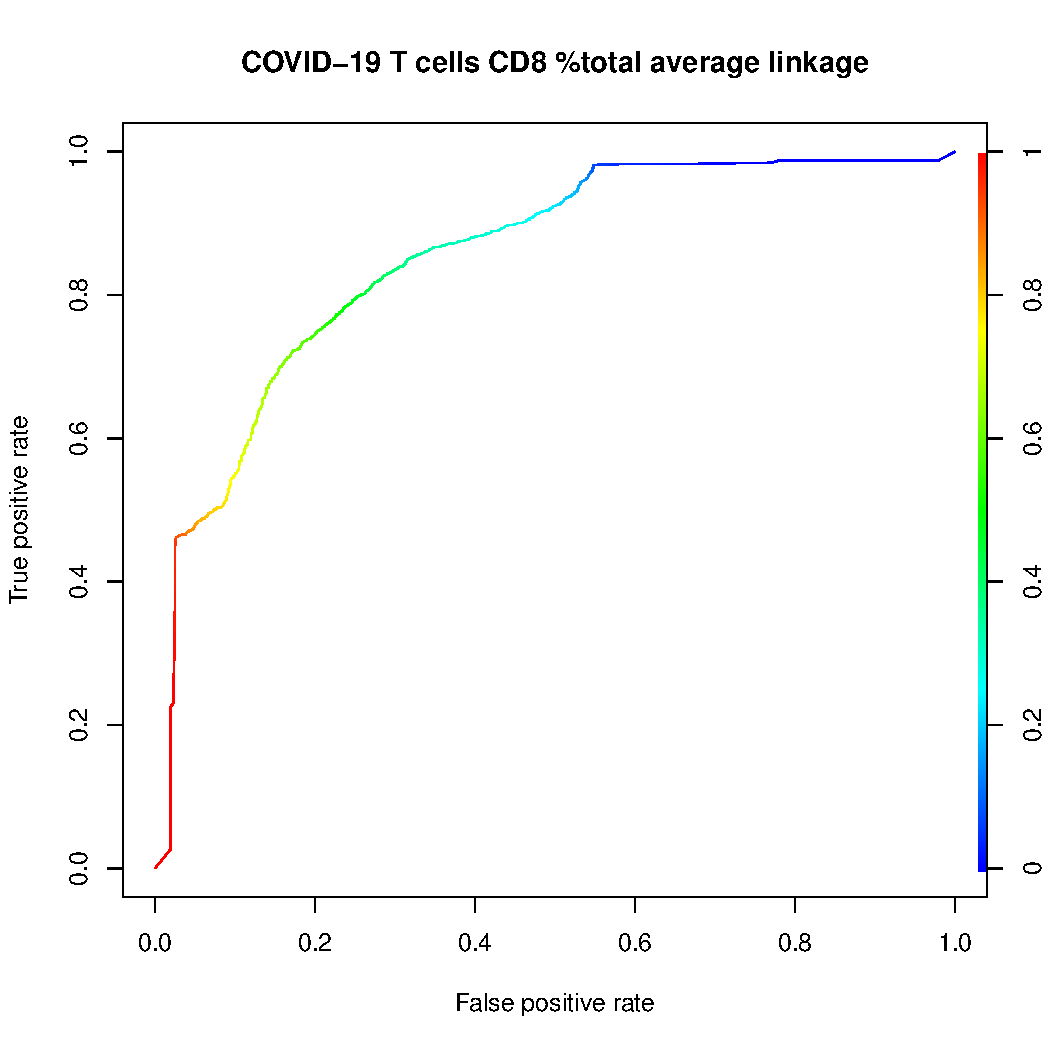
\includegraphics[width=\maxwidth]{figure/fig_code-11} 

\includegraphics[width=\maxwidth]{figure/fig_code-12} 

\includegraphics[width=\maxwidth]{figure/fig_code-13} 

\includegraphics[width=\maxwidth]{figure/fig_code-14} 

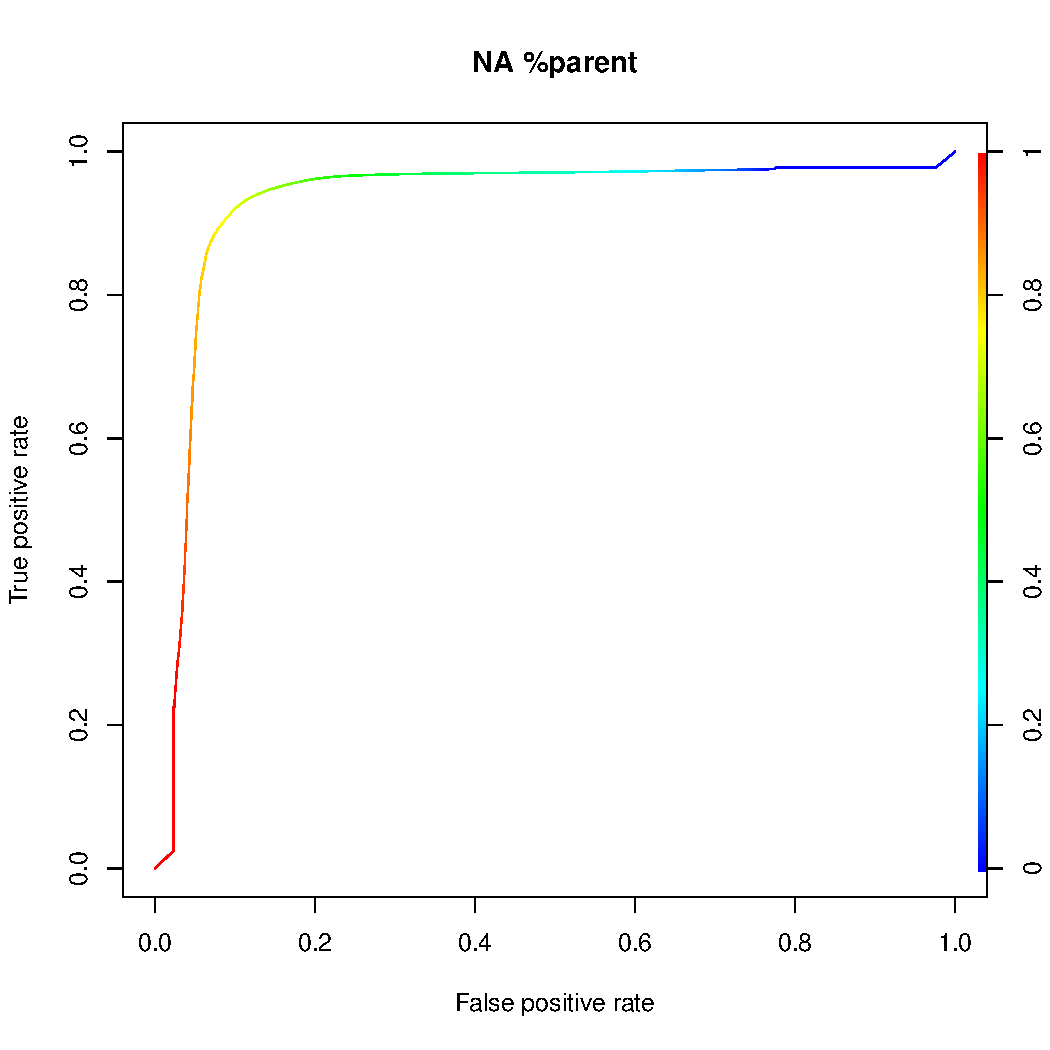
\includegraphics[width=\maxwidth]{figure/fig_code-15} 

\includegraphics[width=\maxwidth]{figure/fig_code-16} 

\includegraphics[width=\maxwidth]{figure/fig_code-17} 

\includegraphics[width=\maxwidth]{figure/fig_code-18} 

\includegraphics[width=\maxwidth]{figure/fig_code-19} 

\includegraphics[width=\maxwidth]{figure/fig_code-20} 

\includegraphics[width=\maxwidth]{figure/fig_code-21} 

\includegraphics[width=\maxwidth]{figure/fig_code-22} 

\includegraphics[width=\maxwidth]{figure/fig_code-23} 

\includegraphics[width=\maxwidth]{figure/fig_code-24} 

\includegraphics[width=\maxwidth]{figure/fig_code-25} 

\includegraphics[width=\maxwidth]{figure/fig_code-26} 

\includegraphics[width=\maxwidth]{figure/fig_code-27} 

\includegraphics[width=\maxwidth]{figure/fig_code-28} 

\includegraphics[width=\maxwidth]{figure/fig_code-29} 

\includegraphics[width=\maxwidth]{figure/fig_code-30} 

\includegraphics[width=\maxwidth]{figure/fig_code-31} 

\includegraphics[width=\maxwidth]{figure/fig_code-32} 

\includegraphics[width=\maxwidth]{figure/fig_code-33} 

\includegraphics[width=\maxwidth]{figure/fig_code-34} 

\includegraphics[width=\maxwidth]{figure/fig_code-35} 

\includegraphics[width=\maxwidth]{figure/fig_code-36} 
\end{knitrout}


\begin{figure}
\begin{knitrout}
\definecolor{shadecolor}{rgb}{0.969, 0.969, 0.969}\color{fgcolor}\begin{kframe}


{\ttfamily\noindent\color{warningcolor}{\#\# Warning in ncases * ncontrols: NAs produced by integer overflow}}\end{kframe}
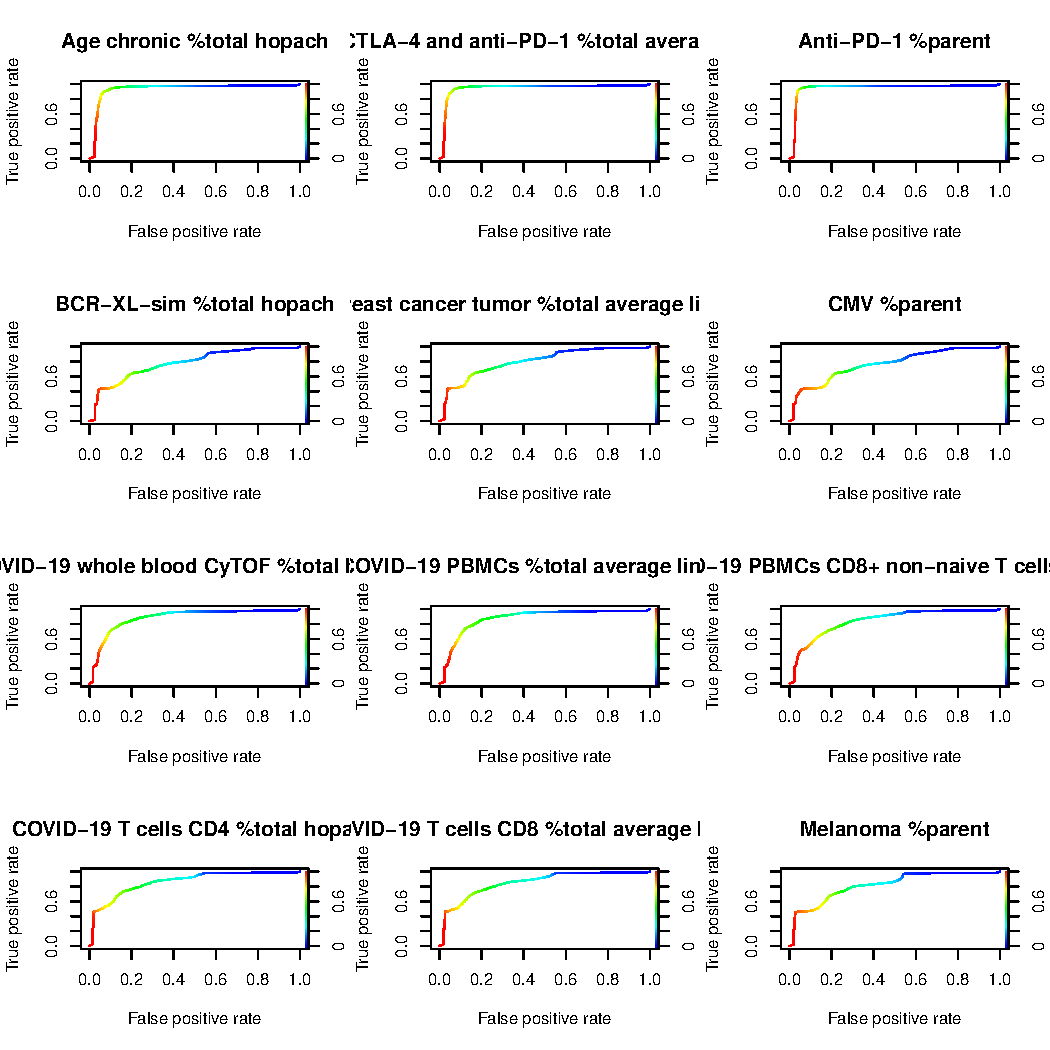
\includegraphics[width=\maxwidth]{figure/unnamed-chunk-1-1} 

\includegraphics[width=\maxwidth]{figure/unnamed-chunk-1-2} 

\includegraphics[width=\maxwidth]{figure/unnamed-chunk-1-3} 
\begin{kframe}\begin{verbatim}
## NULL
\end{verbatim}
\end{kframe}
\end{knitrout}
\title{ROC curves of datasets 1-4.\label{fig:1}}
\end{figure}

\begin{figure}
\begin{knitrout}
\definecolor{shadecolor}{rgb}{0.969, 0.969, 0.969}\color{fgcolor}\begin{kframe}


{\ttfamily\noindent\color{warningcolor}{\#\# Warning in ncases * ncontrols: NAs produced by integer overflow}}\end{kframe}
\includegraphics[width=\maxwidth]{figure/unnamed-chunk-2-1} 

\includegraphics[width=\maxwidth]{figure/unnamed-chunk-2-2} 

\includegraphics[width=\maxwidth]{figure/unnamed-chunk-2-3} 
\begin{kframe}\begin{verbatim}
## NULL
\end{verbatim}
\end{kframe}
\end{knitrout}
\title{ROC curves of datasets 5-8.\label{fig:2}}
\end{figure}

\begin{figure}
\begin{knitrout}
\definecolor{shadecolor}{rgb}{0.969, 0.969, 0.969}\color{fgcolor}\begin{kframe}


{\ttfamily\noindent\color{warningcolor}{\#\# Warning in ncases * ncontrols: NAs produced by integer overflow}}\end{kframe}
\includegraphics[width=\maxwidth]{figure/unnamed-chunk-3-1} 

\includegraphics[width=\maxwidth]{figure/unnamed-chunk-3-2} 

\includegraphics[width=\maxwidth]{figure/unnamed-chunk-3-3} 
\begin{kframe}\begin{verbatim}
## NULL
\end{verbatim}
\end{kframe}
\end{knitrout}
\title{ROC curves of datasets 9-12.\label{fig:3}}
\end{figure}


- provide Benchmarking plots, once using balanced accuracy as a measure of comparison, once using our "own"
- report findings / observations

%%%%%%%%%%%%%%%%%%%%%%%%%%%%%%%%%%%%%%%%%%%%%%%%%%%%%%%%%%%%%%%%%%%%%%

% LaTeX file for Chapter 05


% 
\chapter{Discussion}\label{sec:discussion}

part I:
- why does our analysis look different from theirs?
- what has remained unclear?
- what could be explored further?

part II: 
- why does our analysis look different than theirs?
- are there differences when using other measure instead of balanced accuracy? why? what does that mean?
- what remains unclear?
- what could be explored further?

%%%%%%%%%%%%%%%%%%%%%%%%%%%%%%%%%%%%%%%%%%%%%%%%%%%%%%%%%%%%%%%%%%%%%%
\appendix

% LaTeX file for Chapter 01



\chapter{Appendix}

- code
- where the data can be found
\cleardoublepage

%%%%%%%%%%%%%%%%%%%%%%%%%%%%%%%%%%%%%%%%%%%%%%%%%%%%%%%%%%%%%%%%%%%%%%
\phantomsection  % needed to create a link to here for hyperref
\addtocontents{toc}{\protect \vspace*{10mm}}
\renewcommand\bibname{References}              % Comment if you want `Bibliography' as title
\addcontentsline{toc}{chapter}{\bfseries \bibname}

\bibliographystyle{mywiley} 
\bibliography{biblio}

\cleardoublepage

\end{document}

